% A complete, compilable §I-P1 "pipeline-with-hero" method figure.
% Build:  pdflatex pipeline_hero.tex   ->  pipeline_hero.pdf
% Then in your paper:  \includegraphics[width=\linewidth]{pipeline_hero.pdf}
% (The main document never touches tikzpicture -> zero compile risk.)
\documentclass[tikz,border=3mm]{standalone}
\usepackage{times}
\usetikzlibrary{positioning, arrows.meta, fit, backgrounds, shapes.geometric, calc}
\begin{document}
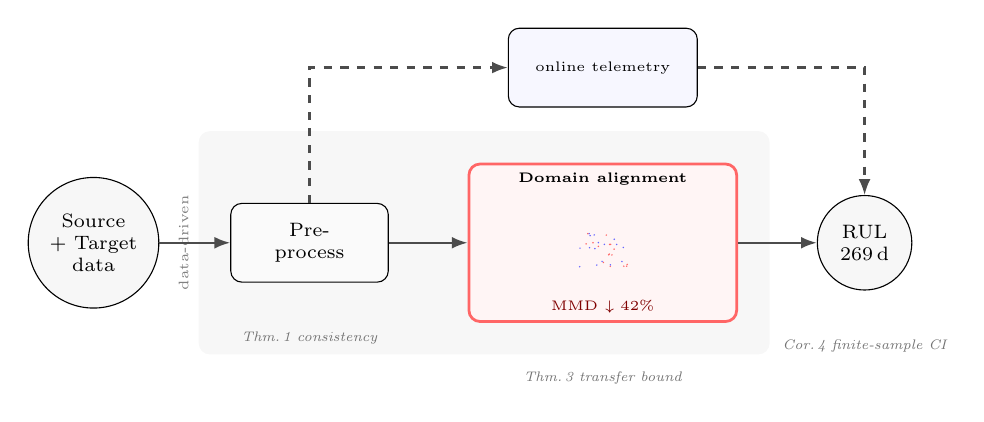
\begin{tikzpicture}[
  io/.style   = {circle, draw, minimum size=12mm, align=center, font=\scriptsize, fill=black!3},
  proc/.style = {rectangle, draw, rounded corners, minimum height=10mm,
                 minimum width=20mm, align=center, font=\scriptsize, fill=black!2},
  hero/.style = {rectangle, draw=red!60, line width=1pt, fill=red!4,
                 rounded corners, align=center},
  arr/.style  = {-{Latex[length=2mm]}, thick, gray!60!black},
  thm/.style  = {font=\tiny\itshape, text=black!55},
]
  % --- main pipeline: input -> preprocess -> [HERO] -> output ---------------
  \node[io] (in) {Source\\+ Target\\data};
  \node[proc, right=9mm of in] (pre) {Pre-\\process};

  % HERO band: embed the REAL method object (source/target scatter, aligned)
  \node[hero, right=10mm of pre, minimum width=34mm, minimum height=20mm] (hero) {};
  \node[font=\tiny, anchor=north] at (hero.north) {\textbf{Domain alignment}};
  \begin{scope}[shift={($(hero.center)+(0,-1mm)$)}]
    % source cloud (blue) and target cloud (red), overlapping after alignment
    \foreach \i in {1,...,16}{
      \pgfmathsetmacro{\sx}{0.32*rand} \pgfmathsetmacro{\sy}{0.22*rand}
      \fill[blue!60] (\sx,\sy) circle (0.3pt);
      \pgfmathsetmacro{\tx}{0.32*rand} \pgfmathsetmacro{\ty}{0.22*rand}
      \fill[red!60] (\tx,\ty) circle (0.3pt);
    }
  \end{scope}
  \node[font=\tiny, anchor=south, text=red!50!black] at (hero.south) {MMD $\downarrow42\%$};

  \node[io, right=10mm of hero] (out) {RUL\\$269$\,d};

  \draw[arr] (in) -- (pre);
  \draw[arr] (pre) -- (hero);
  \draw[arr] (hero) -- (out);

  % --- top bypass lane (online / streaming) ---------------------------------
  \node[proc, above=7mm of hero, minimum width=24mm, fill=blue!3, font=\tiny] (online) {online telemetry};
  \draw[arr, dashed] (pre.north) |- (online.west);
  \draw[arr, dashed] (online.east) -| (out.north);

  % --- bottom guarantee band (theorem / metric anchored under each block) ----
  \node[thm, below=5mm of pre]  {Thm.\,1 consistency};
  \node[thm, below=5mm of hero] {Thm.\,3 transfer bound};
  \node[thm, below=5mm of out]  {Cor.\,4 finite-sample CI};

  % swimlane frame behind the data-driven stretch
  \begin{scope}[on background layer]
    \node[fit=(pre)(hero), draw=none, fill=black!3, rounded corners,
          inner sep=4mm, label={[font=\tiny, text=black!50]left:\rotatebox{90}{data-driven}}] {};
  \end{scope}
\end{tikzpicture}
\end{document}
